% Chapter3.tex
\chapter{WebDoc - Web Application Documentor}\label{ch:CP}

\begin{figure}[h]
    \centering
    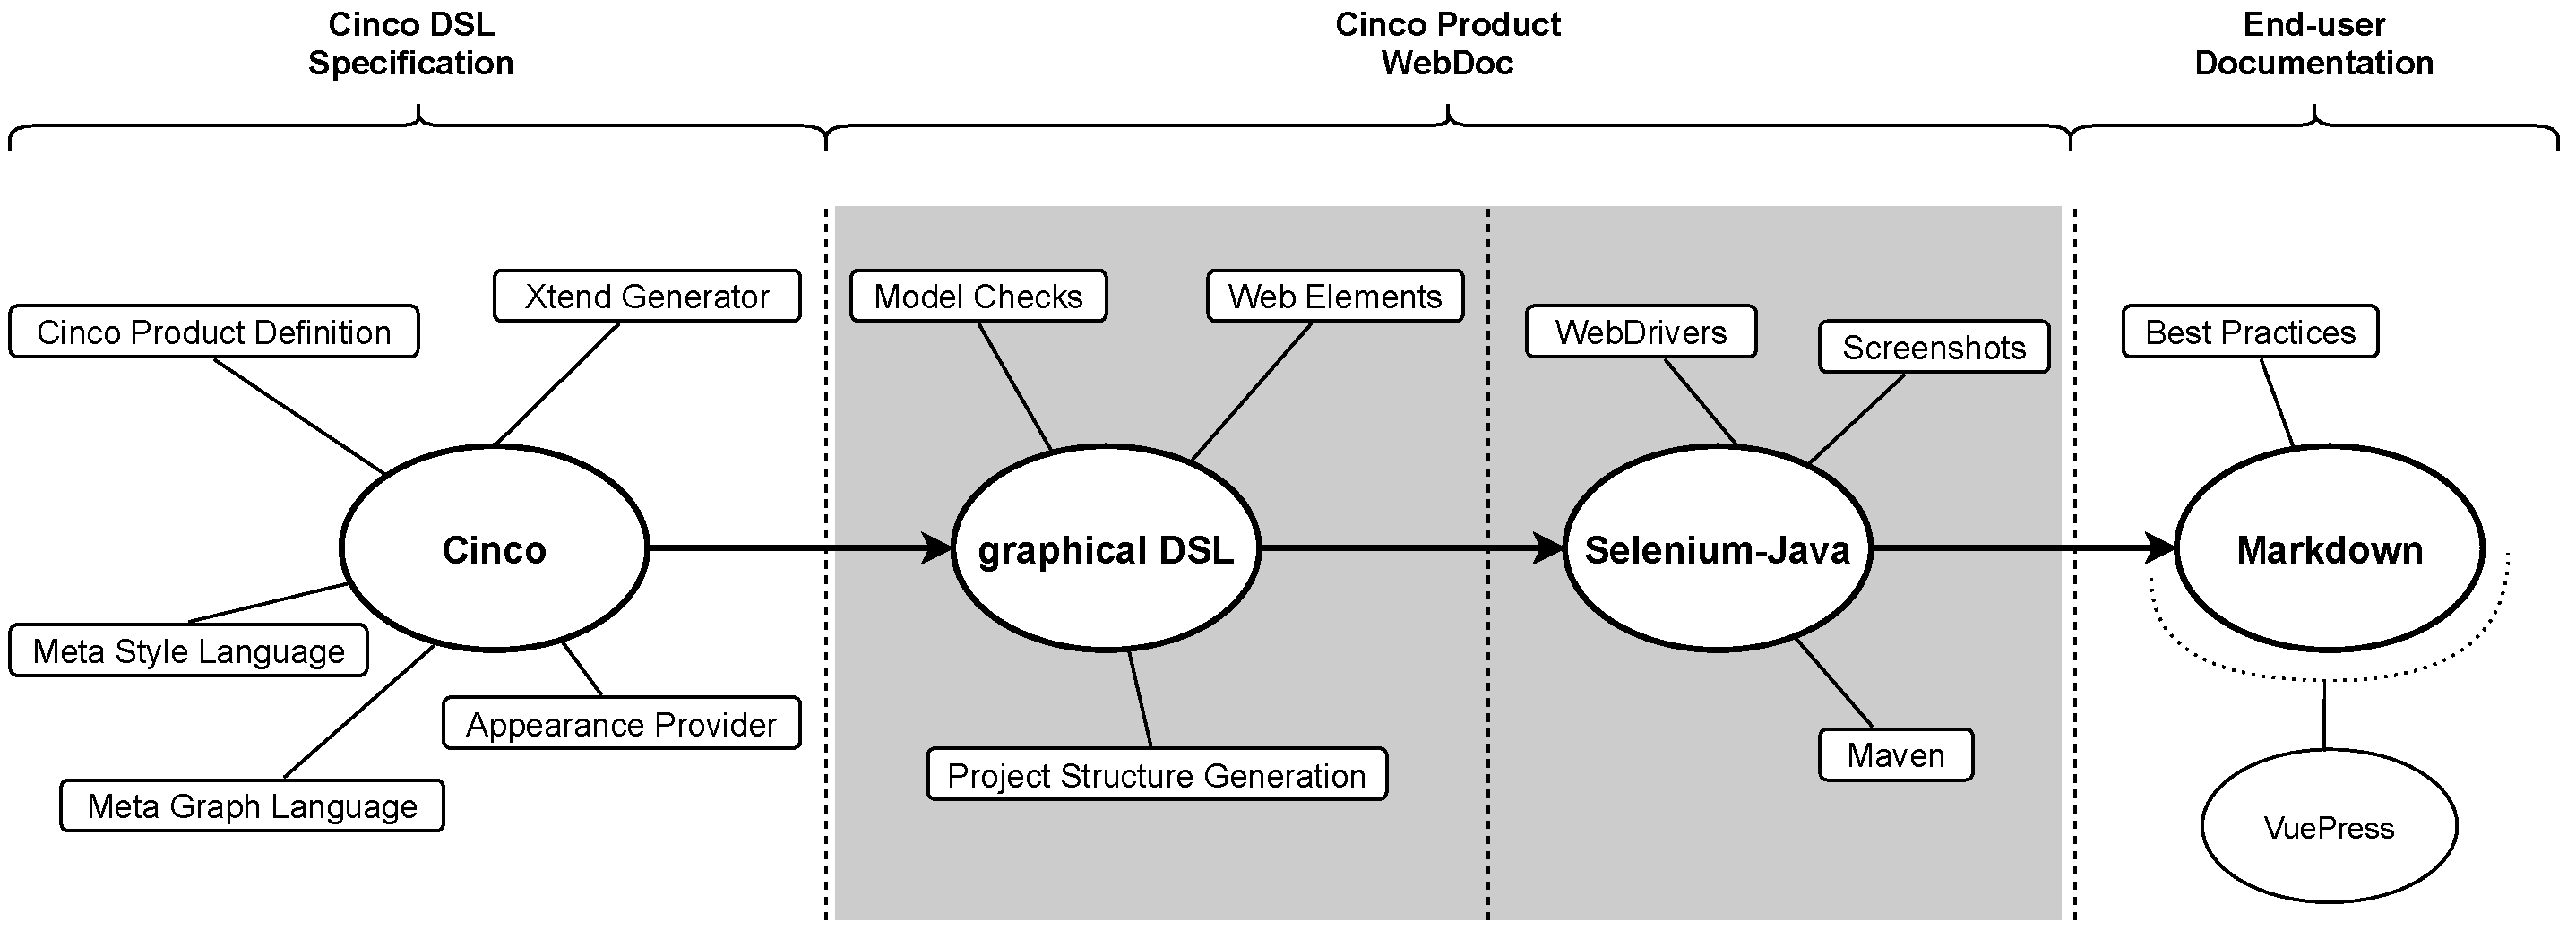
\includegraphics[width=\textwidth]{WebDocDevelopment-gDSL.pdf}
    \label{fig:webDoc}
\end{figure}

Having described the \textsc{Cinco} DSL specification of the graphical modeling tool, we come now to the description of the model editor instantiated from it. First, we give a succinct explanation of our graphical DSL, then illustrate the fundamental building blocks of our documentation model and by presenting at the same time our \textsc{Cinco} product: WebDoc\footnote{GitHub repository: \url{https://github.com/MukendiMputu/UserDoc}}. Later, we demonstrate the use of these graphical elements to model a specific user workflow on the website we want to document. At the end, we show how using the editor built-in generator, we generate the target application that generate the Markdown files to be shown in the Web browser.

\section{Graphical DSL}\label{sec:gDSL}

Our graphical DSL mainly comprises node elements, which have been applied different appearances to, must resemble to some extent the corresponding Web elements they represent, as well as connector elements to connect the nodes to sequence graphs. The purpose behind this approximated replication is not to recreate all possible Web elements, but to give the developer a sense of control over the interactable UI elements. With those elements at hand, the designer can simply model a user action by arranging node elements following the navigation path of the Web application. This graphical language is in such way domain specific, that it is tailored for modeling Web applications inside a Web browser; modeling a documentation for a desktop application for example would not be possible.

\section{Graph Editor}\label{sec:graphEditor}

The WebDoc editor is mainly composed of the canvas in the middle of the working environment (1), where the developer can drag and drop model elements from the palette located on the right-hand side (2). Herein, elements are grouped in categories. On the left-hand side we have the project explorer showing the current project structure (3). The main model files have the extensions .doc and .feat, where the latter is the entry point of the documentation application.

\begin{figure}[h]
    \centering
    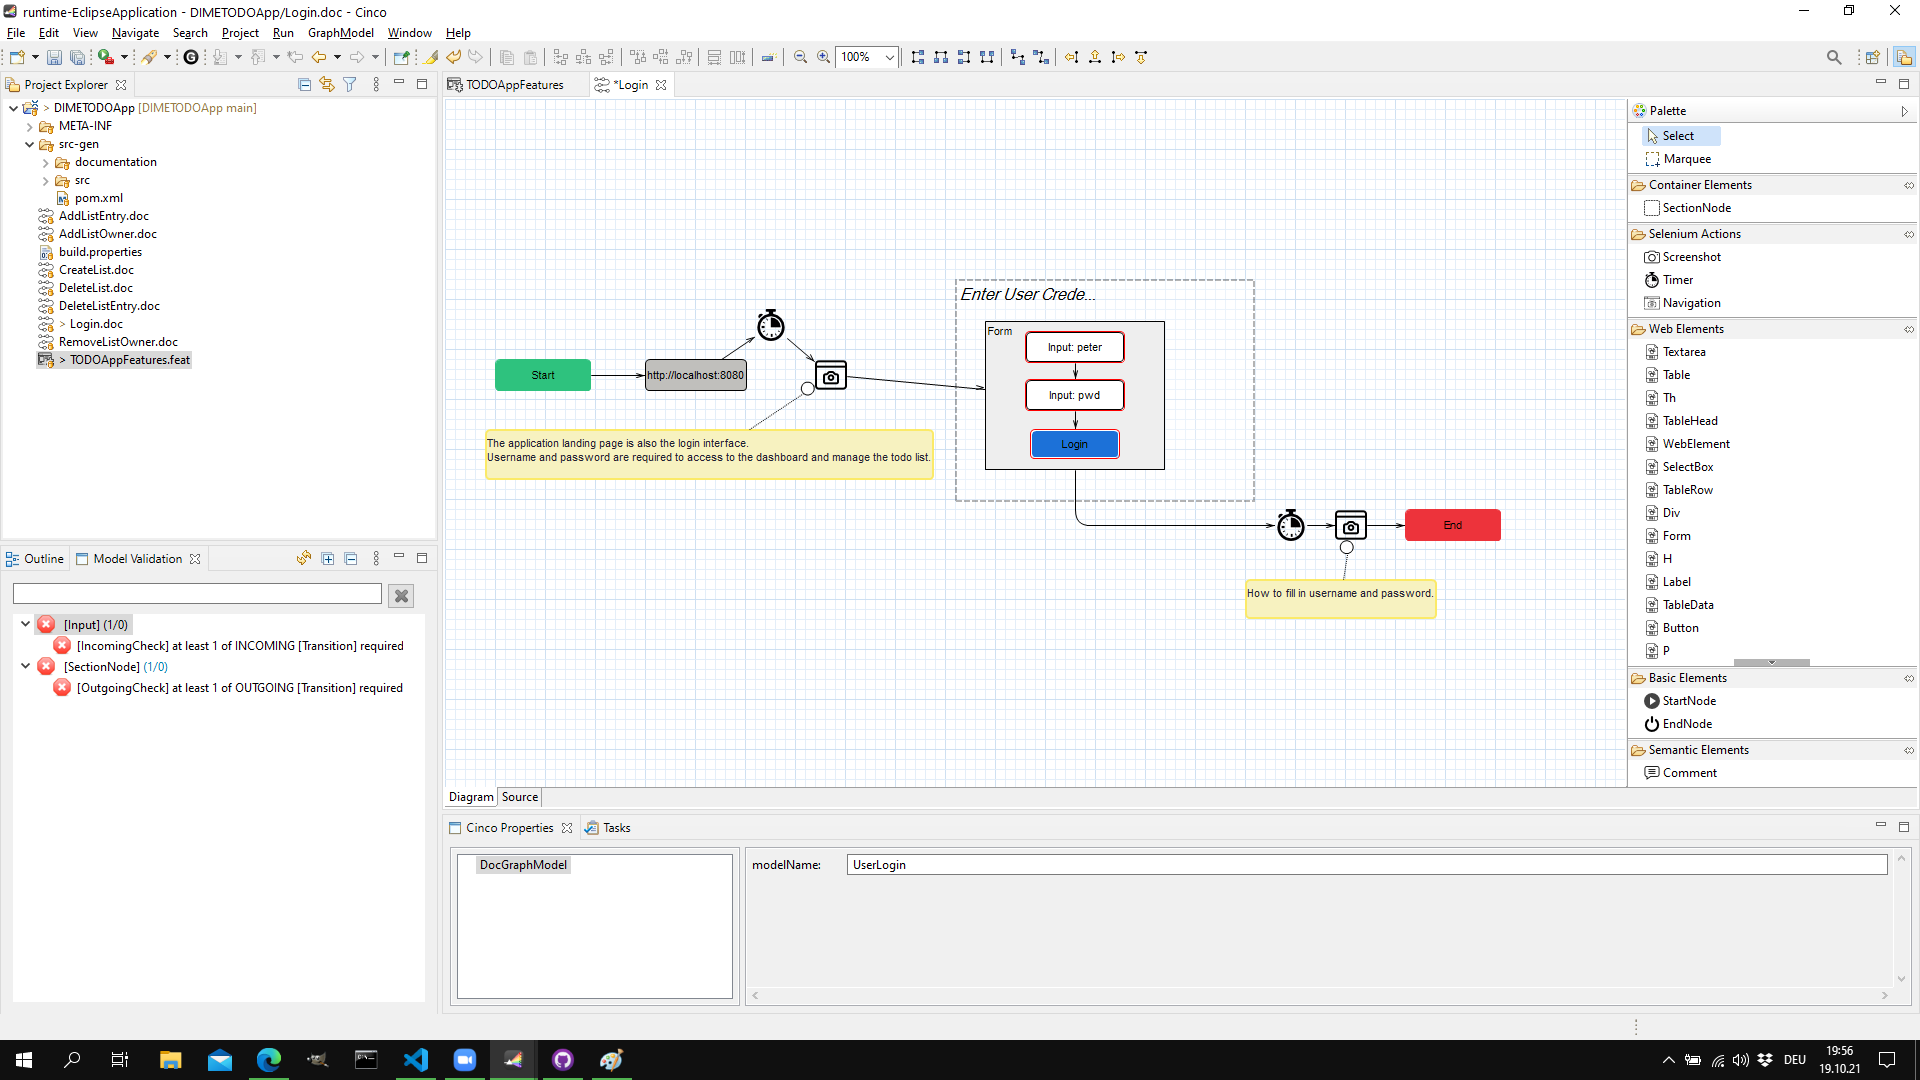
\includegraphics[width=\textwidth]{DocGraphModelChecks.png}
    \caption{\textsc{Cinco} Product Application - Graph model editor}\label{fig:graphDSL}
\end{figure}

All diagrams that are open in the editor are checked in the background for compliance with the requirements described on the metalevel and shown in the Model Checking view right beneath the project explorer (4). There is also the \textsc{Cinco} property view (5) that displays the attributes and values of any selected element in the editor. This is where the developer can modify those values if the attribute field allows it.

\section{WebDoc's Model Elements}\label{sec:WebDocModelElem}

On a Web page rendered in the Web browser, there is a small amount of HTML elements the user can interact with. Most of them resides within the HTML forms, tools that are used for collecting data from the user or allowing them to control a user interface~\cite{mozillaMDN}. Input fields (of all types: text, password, textarea, checkbox, etc.) and buttons are the prominent ones. Those are the Web elements that primarily constitute the palette of our model elements. In the previous chapter, we defined two different \glsplural*{mgl}: one for modeling the Web application features and the other one for modeling the user actions that make up those features.

\subsection{FeatureGraphModel}\label{sec:FeaGrahptModElem}

The FeatureGraphModel is the application starting point specified by the \lstinline{feature.mgl}. Here, the developer groups all the features that needs to be documented in feature containers. Figure~\ref{fig:featGraph} shows a sample of the features modeled for our task management application, including the ability to login, create a new list, add or remove a task from that list, and finally delete the entire list. The documentation website's resulting sidebar is depicted in Figure~\ref{fig:sidebar}, albeit it should be noted that the "Introduction" is not an application feature, but rather the introductory page displaying the various functionalities. Moreover, our application offers the possibility to also add a new list owner, which already exist in the system as regular user.

On the top left-hand corner, you can see an property container holding the WebDriver property, whose value is set to \lstinline[language=MGL]{FIREFOX}. It is one of the additional model elements that help the developer define configuration that otherwise could not be modeled, but still essential for the execution of the application. This property value will be assigned to the Selenium WebDriver variable in the Java class. Remember that the executable file for the chosen WebDriver must already exist somewhere in file system and the path to it must be specified here in the property view.

\begin{figure}[H]
    \begin{subfigure}[b]{0.5\textwidth}
        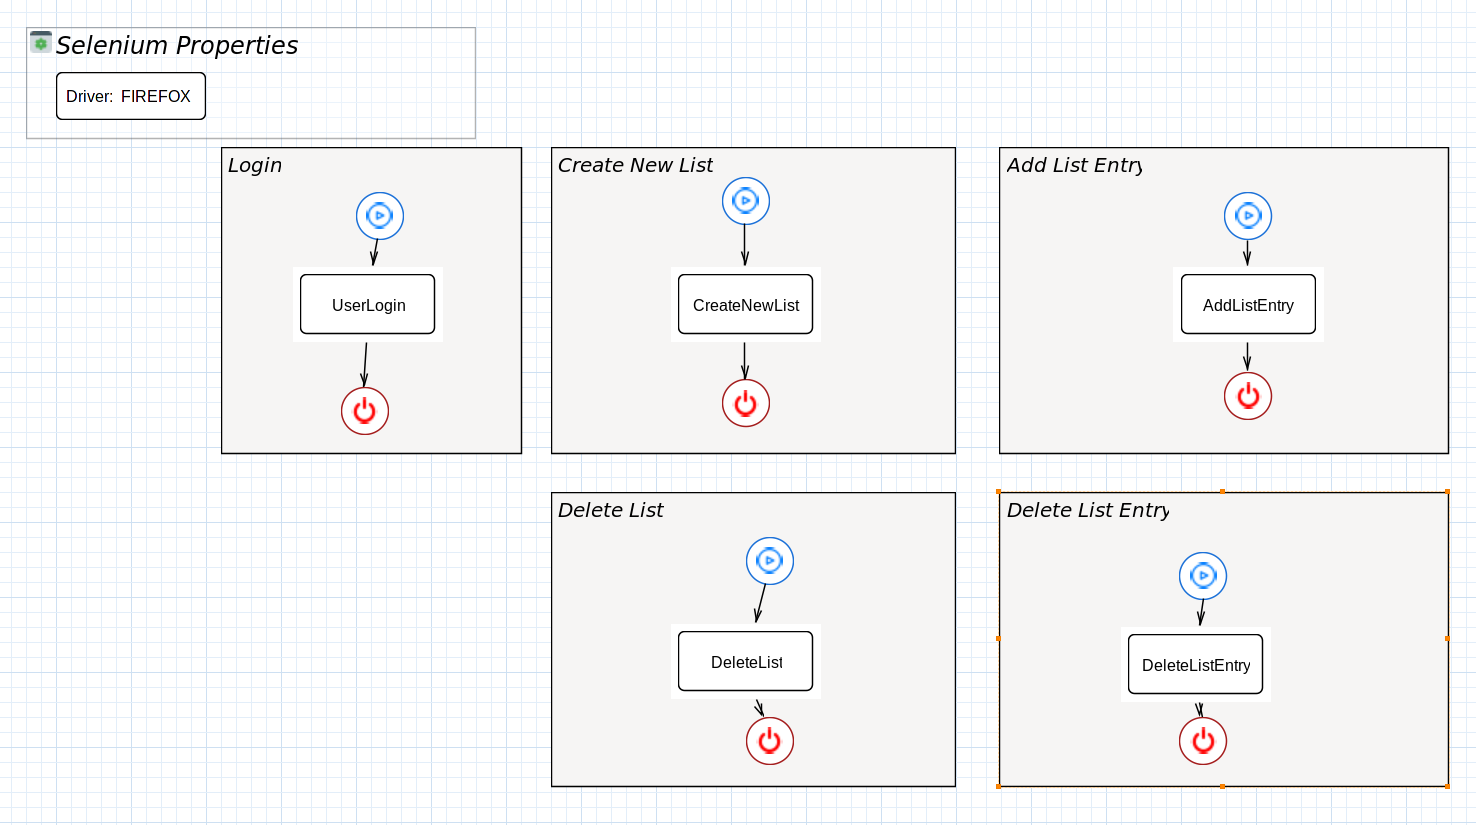
\includegraphics[width=\textwidth]{FeatureGraphModel2.png}
        \caption{Features in the FeatureGraphModel}
        \label{fig:featGraph}
    \end{subfigure}
    ~
    \begin{subfigure}[b]{0.5\textwidth}
        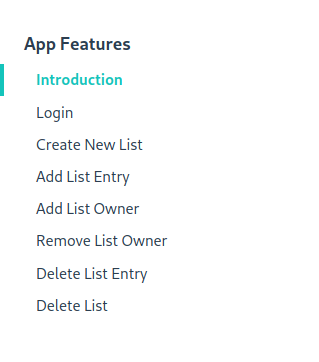
\includegraphics[width=\textwidth]{Sidebar.png}
        \caption{Menu structure on the documentation website}
        \label{fig:sidebar}
    \end{subfigure}
\end{figure}

Despite the fact that the features are provided in a logical workflow order, they are still distinct from one another and will be generated separately. As indicated in the last chapter, however, this separation does not preclude reusability, as it is feasible to embed one whole DocGraphModel within another. Consider the CreateNewList functionality, which necessitates the user being signed in in order to create a new task list. So, instead of repeating the login sequence in this one, the documentation developer may simply drag and drop the UserLogin.doc file into the diagram of the new model graph and connect it to the sequence as if it were a regular graph node. (see figure~\ref{fig:reusability}). When you double-click on an imported subgraph, you'll be sent straight to the original graph model. This double-click action was implemented by annotating the associated node specification with the \lstinline[language=MGL]{@doubleClickAction} annotation and providing a custom action class that holds the implementation logic. Furthermore, by unchecking the createScreenshots checkbox in the property view of a subgraph, the designer can disable the creation of screenshots for that specific model, which is enabled by default. This prevents the same screenshot from being taken several times when the subgraph is reused.

\begin{figure}[h]
    \centering
    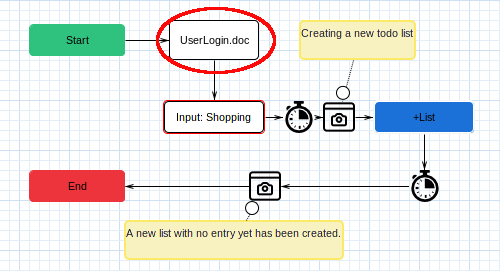
\includegraphics[width=0.75\textwidth]{Reusability.png}
    \caption{\textsc{Cinco} product - Reusing Login graph model in the CreateNewList graph model}
    \label{fig:reusability}
\end{figure}

The semantic elements in the feature graph model are incorporated into the underlying featureContainers for simplicity's sake. When you click on a featureContainer like this, it opens the Cinco property view, which includes a multiline input form called 'description.' This is where the documentation designer can offer text content for the Markdown documentation files while also providing descriptive text for the diagram objects. These information texts will be gathered during the code creation process to create the complete documentation text.

\subsection{DocGraphModel}\label{sec:DocGrahpModElem}

Figure~\ref{fig:loginSeq} illustrates the steps a user would take to log into our example Web application, as well as the Web elements that will be interacted with. They create the user login sequence for our Web application when connected in a logical sequence.

\begin{figure}[h]
    \centering
    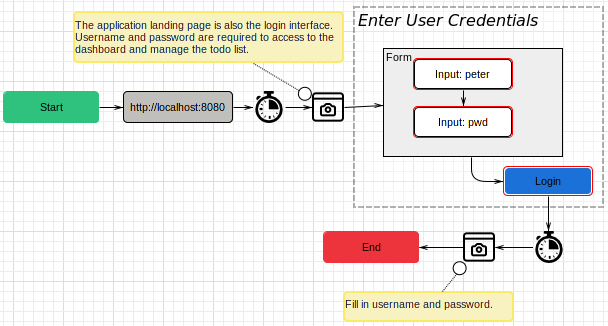
\includegraphics[width=0.85\textwidth]{WebDoc-graphModel.png}
    \caption{Example of a user workflow: here the login sequence}
    \label{fig:loginSeq}
\end{figure}

The sequence begins with the start node, which is the starting point of every user sequence, then comes the navigation node, used to navigate from one Web page to another. Next, the timer node waits explicitly for an amount of second  determined by the designer in the property view and for a certain condition to become true before continuing. Those ExpectedConditions are i.e., \lstinline{presenceOfElementLocated}, \lstinline{elementToBeClickable}, just to name a few. If we take for example the condition \lstinline{presenceOfElementLocated}, the timer holds the WebDriver execution for 3 seconds, checking every 500 milliseconds if the targeted Web element appears on the page. This is a necessary step to capture all elements of the page while taking the screen capture, as some elements take time to be completely loaded. Right after the timer comes the Screenshot node, that captures the current application state, displaying the application landing page, which also is the login pane. In the property view, one can give a unique file name to each image to be saved. The comment node allows the documentation creator to add descriptive text about the picture, that will be later added to the Markdown file as image caption. Next comes the Section node, that regroups form elements for entering and validating user credentials. As you can see, all input nodes, as well as the button node, have a red border that represents the highlighted state of the element. The model designer may see which elements will be highlighted in the following screenshot, after which the login sequence will end. 

The purpose of the Web element nodes is to allow the concrete \gls*{html} elements in the browser to be addressed. This implies that appropriate actions can be applied to such a representation of an \gls*{html} element. Considering for instance the input field in the picture below, the action of typing in a text is made possible by providing a property variable \lstinline{content}, whose value is then display inside the node element (here i.e. ''peter'' and ''pwd''). The same holds true for button elements, which can be applied the click action or for selectboxes, which can be dropped down to reveal the options they contain, etc. In addition to that, all Web elements can be highlighted either by setting the \lstinline{highlighted} property to true or by letting the Highlight node under the \textit{Selenium Actions} category take care of it. The screenshot taken immediately after will have that specific element surrounded with a red border as well (see fig.~\ref{fig:screenshot}).

\begin{figure}[h]
    \centering
    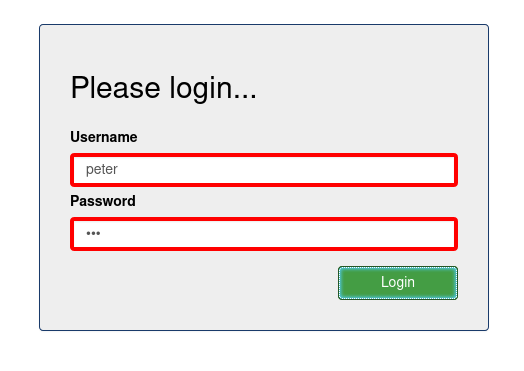
\includegraphics[width=0.55\textwidth]{ApplicationLandingPage.png}
    \caption{Login pane with screenshot of the highlighted input element}
    \label{fig:screenshot}
\end{figure}

In addition, each node element includes a description attribute, which, as discussed in the preceding section, provides additional content for Markdown files. We decided to hide this attribute in the property view to avoid overcrowding the diagram with semantic components describing each and every node member. All model diagrams are traversed during the generation process, and all descriptive texts are collected into paragraphs, then sections, and finally full Markdown files, depending on the feature they are included in. As a result, the documentation content is organized in the following fashion (see fig.~\ref{fig:markdown}): the featureContainer title is rendered as page headings, the DocGraphModel name is displayed as section headings with all other element descriptions underneath it, and so on.

\begin{figure}[h]
    \centering
    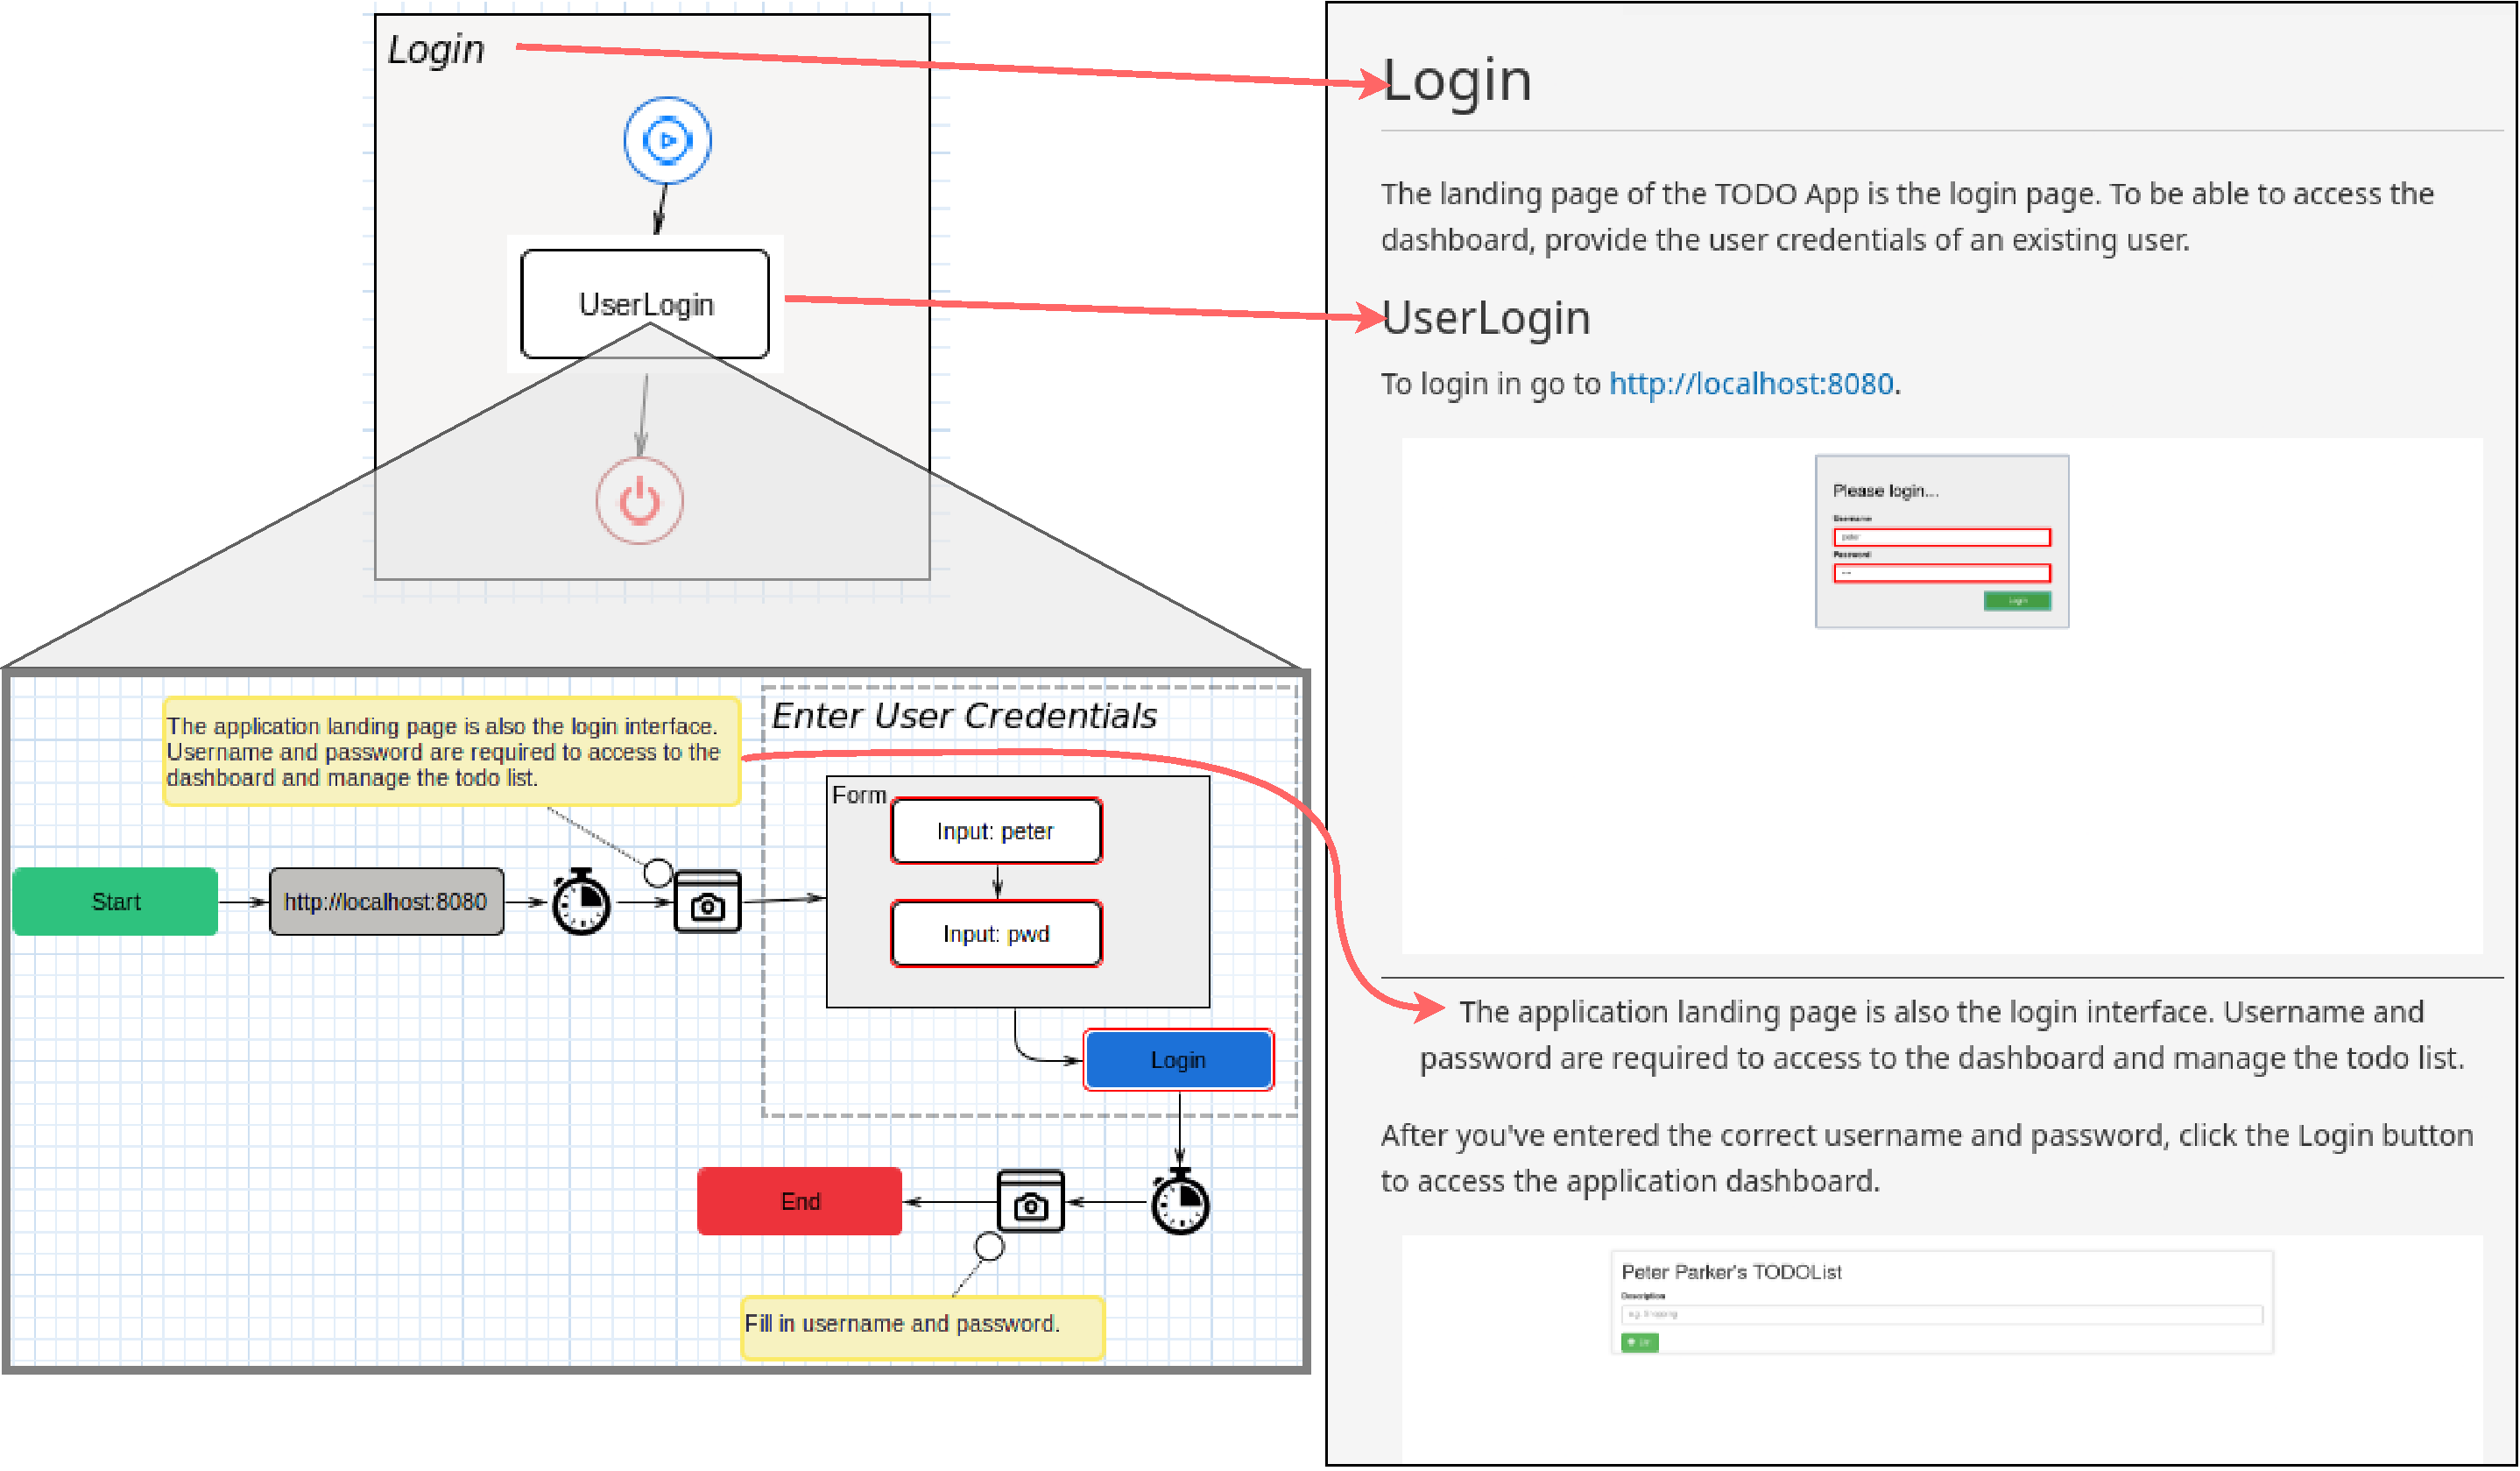
\includegraphics[width=\textwidth]{MardownStructure.pdf}
    \caption{Structural mapping of models to Markdown}
    \label{fig:markdown}
\end{figure}

\section{Graph Model Checks}\label{sec:modCheck}

Modeling valid graph diagrams is crucial for the correctness of the generated application code. Especially the Selenium-Java application code must correctly replicate the user sequence in order capture the correct application state as the user would do. This is particularly daunting if the navigation graph of the underlying Web application is huge.

This means that for each user activity, we must ensure that there is a distinct path and that there is no cycle inside that path. This is reminiscent of various graph theory problems, such as determining whether a path from the start to the end node exists and whether a graph is cycle free. The MCaM plugin, which is incorporated into the \textsc{Cinco} framework, can be used to do this operation~\cite{gitlabcinco}. The plugin must be activated by specifying the \lstinline{@mcam("...")} or the \lstinline{@mcam_checkmodule("...")} annotation with the corresponding parameter in parentheses. 

\begin{figure}[h]
    \centering
    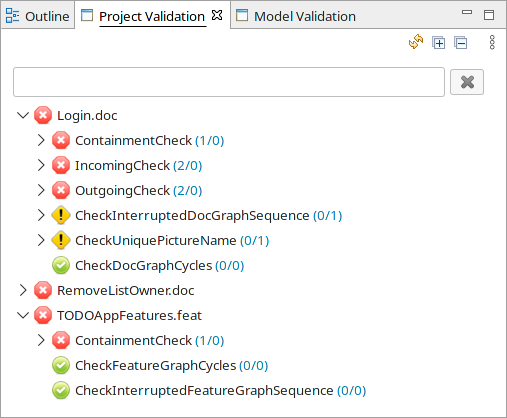
\includegraphics[width=0.7\textwidth]{ProjectValidationView.png}
    \caption{Project Validation view showing passed and failed checks}
    \label{fig:modelChecks}
\end{figure}

\subsection{MCaM Check}\label{sec:mcamCheck}

The first one must be declared right above the \lstinline[language=MGL]{graphModel} declaration with the parameter ''check''; this activates the check on the constraints on the graph nodes, for example the multiplicity of the incoming and outgoing edges between them or containment constraints on container nodes, meaning that they can only contain those node elements explicitly specified with the \lstinline[language=MGL]{containableElements} attribute. 

\subsection{MCaM Module Check}\label{sec:mcamModCheck}
The second annotation allows us to specify our own module checks. For instance, we need to ensure that two different screenshot nodes do not bear the same file name or that each sequence starts with the appropriate start node and ends with the end node. We also must ensure that by integrating graph in another one we do not create cycle within the execution path. The \textit{Project Validation} view shows all the checks done on the entire project and marks those that failed or passed the checks accordingly. Figure~\ref{fig:modelChecks} shows for example the checks done on our example project.

\section{Generation Process}\label{sec:GenProcess}

Clicking on this button generates a executable Selenium-Java application, which, once started, runs the user sequence model  as a Selenium script in the Web browser. As mentioned in the preliminary chapter, the generator classes behind this process are written in Xtend, as statically-typed programming language based on Java and translates to Java source code~\cite{Xtend}. 

To be able to start a generation process from a graph model we must declare it ''generatable''. We do so bei adding the \lstinline[language=MGL]{@generatable("path.to.generator.Class")} annotation in the graph model meta-specification. This annotation accepts as parameter a Xtend or Java class that implements the IGenerator, whose \lstinline{generate} method starts the whole process and the path to a location where the generation product will be saved (in our case it is in the \lstinline{src-gen} folder). Recalling the goal we set for application code, we create two folder structures inside the src-gen folder: the first one is the Java project structure with the Selenium script and the second one is the VuePress project holding all the Markdown files with the documentation text. Going deeper into technical details is beyond the scope of this paper, hence we provide an illustration of the whole generation process in figure~\ref{fig:WebDocWorkflow}. As you can see, we begin by designing a graph model in the \textsc{Cinco} product application, the WebDoc editor; clicking on the generate button starts a simultaneous creating of both the aforementioned project files. At this point, a fully functional documentation has already been created. We have chosen to generate the documentation file with references to placeholder pictures, that will be overridden once the Selenium script has been executed. To launch the documentation website two simple commands are needed. Then again, we will not go deeper in details to stay in the scope of our thesis, but there is a great online guide on how to get started with VuePress~\cite{vuepress}. As for the Selenium-Java project, it can be imported in an \glsentryfull{ide} such as Eclipse and launch there. After successful execution, all the placeholder pictures will have been overridden and we have a complete documentation.

\begin{figure}[t]
    \centering
    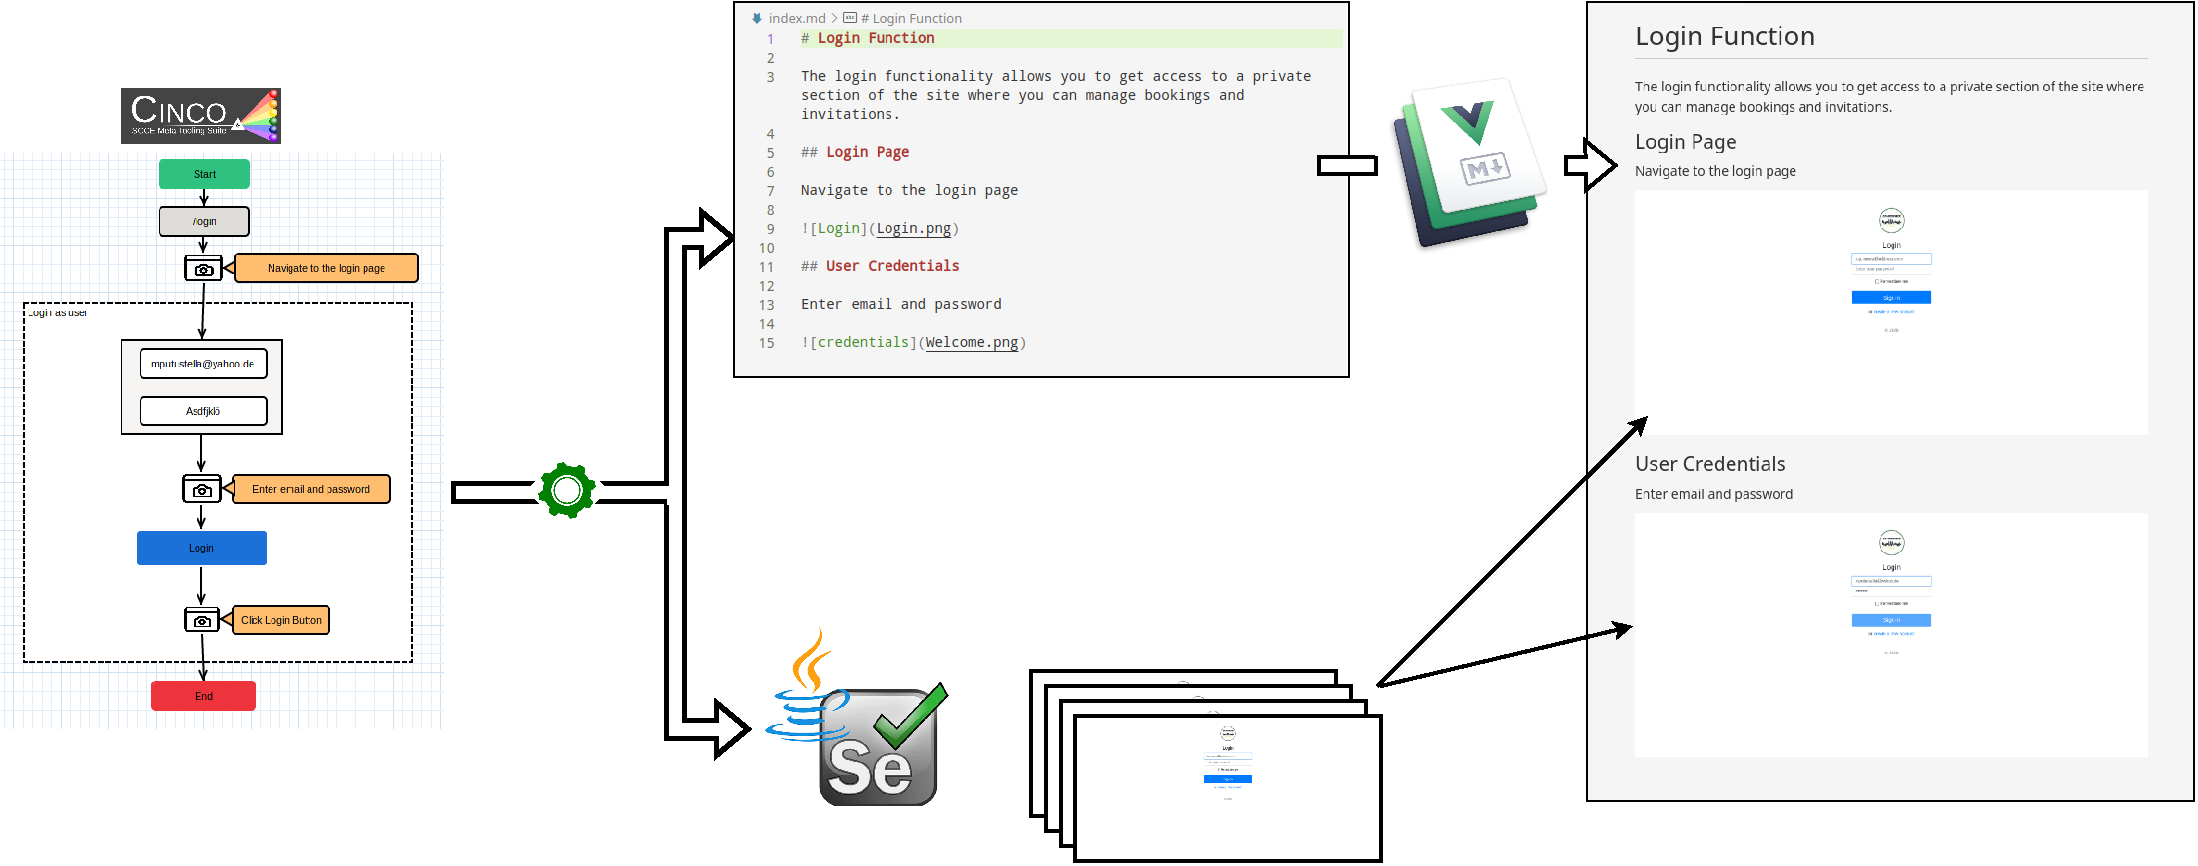
\includegraphics[width=\textwidth]{WebDoc-workflow.pdf}
    \caption{Generation process of End user Documentation}
    \label{fig:WebDocWorkflow}
\end{figure}